\section{PI Control Model} %3.3
At this point, we are equipped with all the building blocks. Let's first recap a PI control model. In PI control, we need to know the value of error and the value of integral of the error. Error is defined by the difference between the nominal value and the signal. In AGC, the nominal value is the nominal frequency in the country (50 Hz or 60 Hz) and the signal is the actual frequency sending into the controller. 

To the integral of the error,  it is should be realised that it is helpful to use discrete mathematics. In discrete mathematics, the value of integral of the error is the accumulated error. Thus, in Python, we can use time-step to help calculating the integral of the error.  Detailedly, in program, we can represent output as 

\begin{figure}[htbp]
\centering
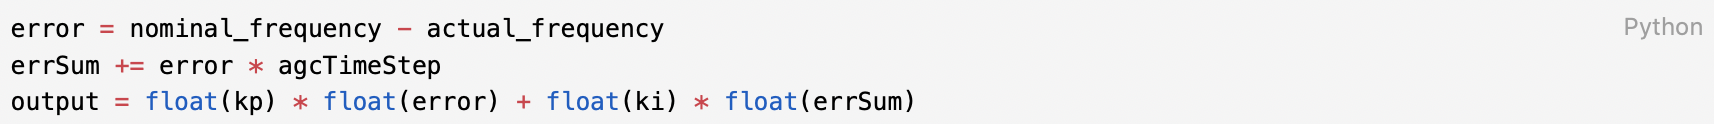
\includegraphics[width = .999\textwidth]{figure/3_3_code1.png}
\caption{Python: PI control algorithm.}
\label{3_3_code1}
\end{figure}

where nominal frequency is 1.0 and we can directly get actual frequency from the simulation. 

Next, we should send output signal to generators through the command, 

\begin{figure}[htbp]
\centering

\includegraphics[width = .999\textwidth]{figure/3_3_code2.png}
\caption{Python: send corrections to the generators.}
\label{3_3_code2}
\end{figure}

where, 'gensName' is the name of generator such as g1, g2 or g9. '1/gensWeight' is $\alpha$ in the Figure~\ref{3_1_Functional}. We use $\alpha$ to ask power proportional to these generators' nominal power.  

Furthermore, we need to consider deadband control. The deadband refers to the the range of input signal when output signal is zero in the domain of transfer signal. In our case, as shown in Figure~\ref{3_3_deadband}, it refers to the range of time when frequency does not change.  

\begin{figure}[htbp]
\centering
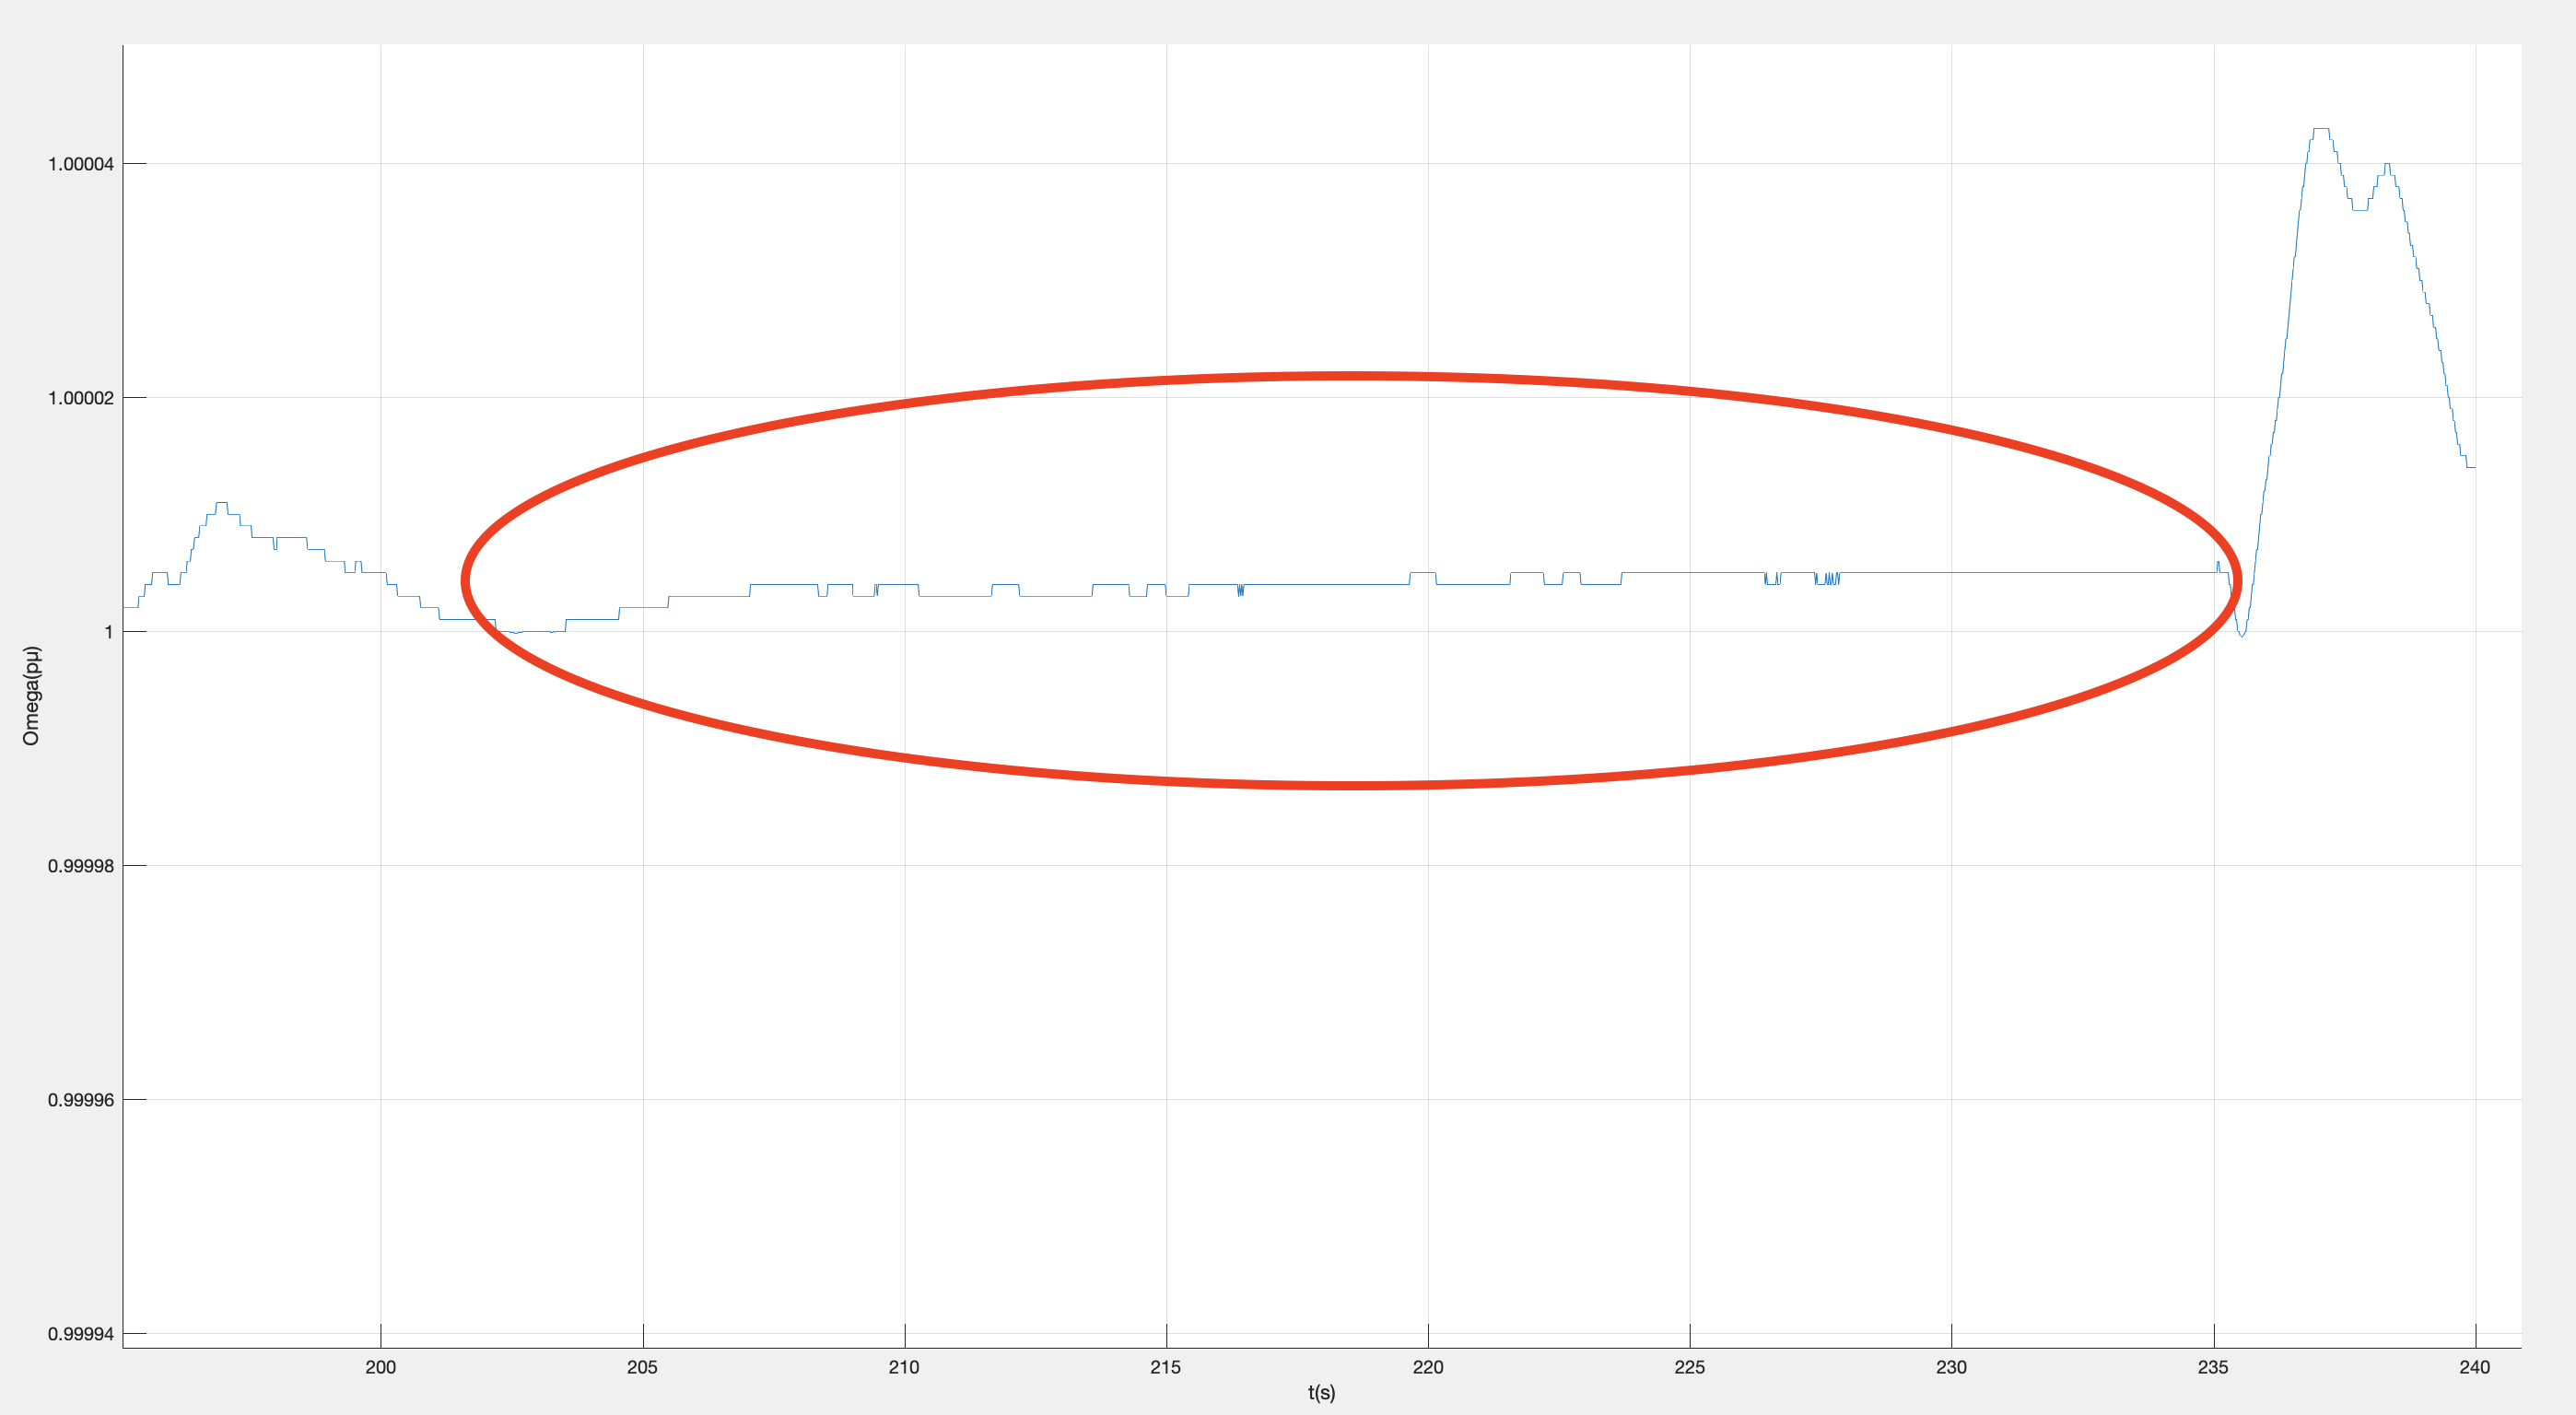
\includegraphics[width = .999\textwidth]{figure/3_3_deadband.png}
\caption{Deadband in SFC.}
\label{3_3_deadband}
\end{figure}


However, in theory, it is impossible to remove deadband totally. The aim to use deadband control is: 
	
    (1). Make the frequency value as small as possible in the deadband area, so we can assume that tiny error is no error;
    
	(2). Make the deadband area as long as possible, so we can keep the frequency in the system stable in a relative long time.  

Thus, we need to choose two parameters in our deadband control: acceptable frequency range in deadband area and control results. 

The acceptable frequency range is a suitable tiny frequency range that we allow deadband occurs. 

For control results, we have three situations. One of them is no deadband control. Another situation is to make error be zero in the deadband area. The last situation is to make the error and the sum of error be zero at the same time.  

\begin{figure}[htbp]
\centering
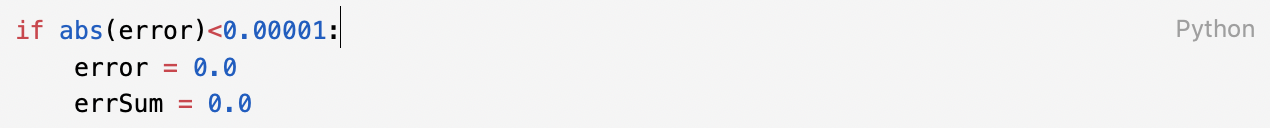
\includegraphics[width = .999\textwidth]{figure/3_3_deadband_code.png}
\caption{Deadband controller.}
\label{3_3_deadband_code}
\end{figure}

Finally, as shown in the Figure~\ref{3_3_deadband_code}, we choose the frequency range in the deadband from -0.000001 Hz to 0.000001 Hz and we make the error and the sum of error be zero at the same time after the deadband control starts. Figure~\ref{3_3_deadband_result} shows the comparison without deadband control and with deadband control. It shows that our deadband control is a more suitable solution for the system. 

\begin{figure}[htbp]
\centering
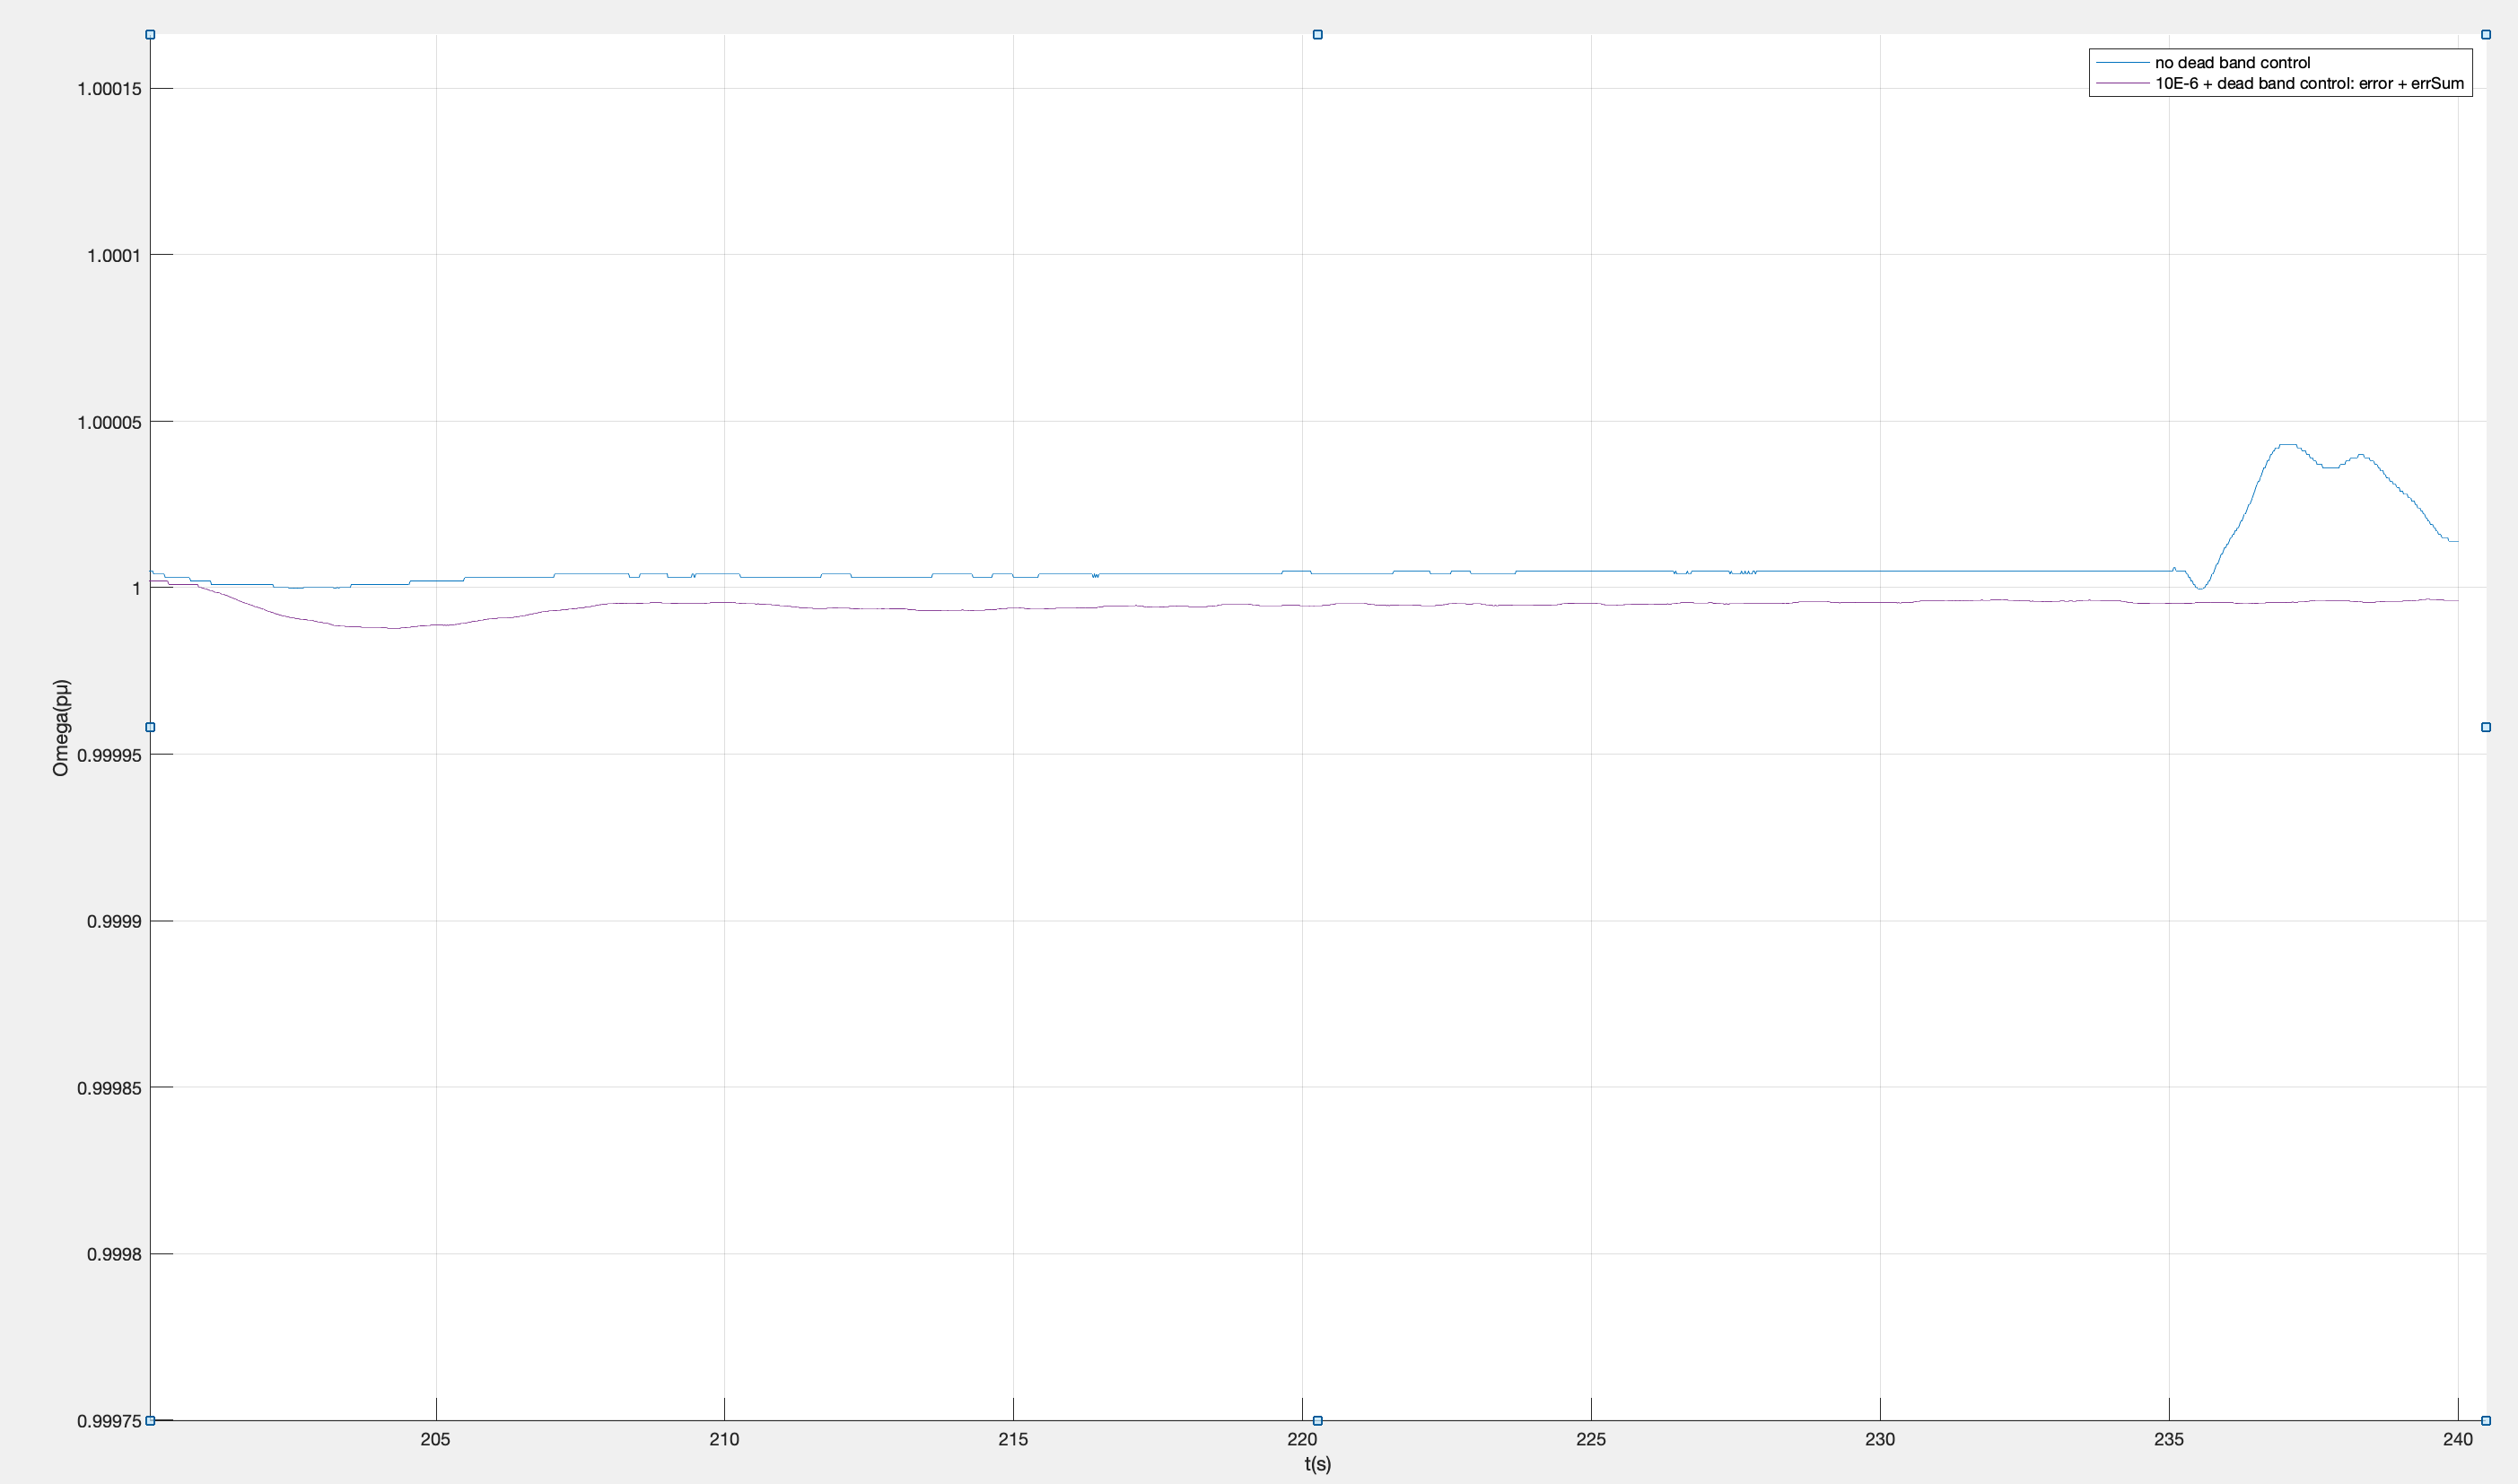
\includegraphics[width = .999\textwidth]{figure/3_3_deadband_result.png}
\caption{Comparison: with and without deadband control.}
\label{3_3_deadband_result}
\end{figure}



We get the input from the existing smart grid simulator and send output to the existing smart grid simulator via our controller. Thus, a communication layer is formed. 

Multiple hard-coded parameters, like the disconnected generator, the generators we asked for their power, amplification factor and time delay, are removed and added into main function so we can test our system comprehensively and easily. 